\documentclass[11pt, a4paper]{article}
%\DeclareUnicodeCharacter{200A}{!!!FIX ME!!!}

\usepackage[utf8]{inputenc}
\usepackage[margin=1in]{geometry}
\usepackage{txfonts}
\usepackage{blindtext}
\usepackage{listings}
\usepackage{hyperref}
\usepackage{graphicx}
\usepackage{xcolor}
\usepackage{cleveref}

\newsavebox{\mybox}
\savebox{\mybox}[0.5\textwidth][c]{aaaa}
%\renewcommand{\lstlisting}{code}
\renewcommand{\lstlistlistingname}{List of codes}
\lstdefinestyle{chstyle}{%
backgroundcolor=\color{gray!12},
basicstyle=\ttfamily\small,
commentstyle=\color{green!60!black},
keywordstyle=\color{magenta},
stringstyle=\color{blue!50!red},
showstringspaces=false,
captionpos = b,
numbers = left,
numberstyle=\footnotesize\color{gray},
numbersep=10pt,
stepnumber=2,
tabsize = 3,
frame=L,
framerule=1pt,
rulecolor=\color{red},
breaklines = true,}


\title{C++ Tutorials for Beginners}
\author{Kouassi Franck Armand Prince}
\date{202024080107}

\begin{document}

\maketitle\hrule
% \begin{center}
% \textbf{C++ Tutorials for Beginners}
% \end{center}
\newpage

\tableofcontents
\listoffigures
\lstlistoflistings
\pagebreak

\section{Getting Started}
%{\blindtext}
This section introduces the basics of C++ programming language and the tools
needed to follow this tutorial. The goal of this tutorial is to help beginners
getting started with C++ programming language. It does not require you to you to
have a prior programming background kownledge. All you have to do is to follow along
with me and and try to \textbf{\textit{WRITE}} the code on your own machine not just read.
Believe me it is easier to read and assume that you have mastered it until you are required
to write the code by yourself, that is where it realize you have not properly understood it.

\subsection{Understand the Computer Language}
%{\blindtext}
Your computer is an incredible and complicated device. Basically, the computer
understands one simple language composed of 0 and 1. Thus a message like this
"\textit{01001100101001010}" could mean "open a window" for instance. Fortunately, we do not have
to learn this language (Binary language). Programmers created languages which are much simpler
than binary language. Here you could check \href{https://en.wikipedia.org/wiki/List_of_programming_languages}
{\emph{\textit{the number of programming languages.}}} \newline
All programming languages have the same goal, that is being able to easily and efficently
communicate with the computer compare to binary language.\newline Here, is how it works :

1. You write the instructions to be executed by the computer in a programming language (e.g C++)

2. The instructions are translated in binary (0 and 1), the language understood by the computer.

3. The computer can now decode the message and executes your request.

\begin{figure}[!ht]
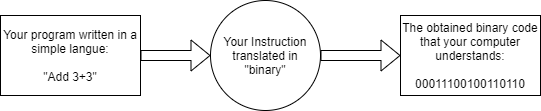
\includegraphics[width = \linewidth]{diagrams/compling.png}
\caption{Compiling Process.}
\label{fig:Compiling Process}
\end{figure}

\subsection{C++ against other programming languages}
Before we start talking about why C++ reprsents a powerful language despite its age. let's discuss the
the key points to analyze before diving into a language.

There exists numerous programming languages as mentioned in above section, although some languages are interesting, 
they are seldom used. The main challenge that comes with these languges, is that they do not have a very big community 
so imagine you working on a project and you are facing a problem, it is difficult to find help since not so many people 
are using the the language.This explains why C++ represents a good choice for debutant programmers. You are not alone, a lot
ressources are availble to guide through your learning process, also C++ is still being widely used.

Another interesting aspect to look at as well is the programming language level. There are of two (02)
types: \textbf{\textit{{high level}}} and \textbf{\textit{{low level}}}.
\newline
\textbf{\textit{{high level}}}: is a language that is that is far from binary language and really
to humans languge,it allows to easily understand and translate instructions contrary to \textbf{\textit{{low level}}}
which a language closed to machine language and generally requires much more effort but gives you more 
control over what you can do, it is a trade-off.

\begin{figure}[!ht]
    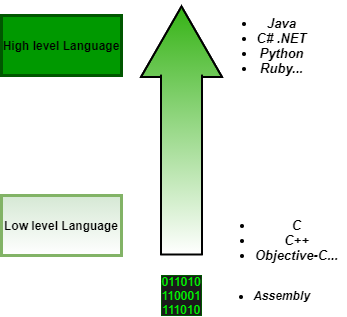
\includegraphics[width = \linewidth]{diagrams/low vs high.png}
    \caption{Programming Language by level.}
    \label{fig:Programming Language by level}
\end{figure}
C++ is a low level language. Do not panic, although coding in C++ might be a little complex, you will 
have in your possession a very \textbf{\textit{{powerful}}} and particulary \textbf{\textit{{fast}}} language.
Infact, if most games are developed in C++, it is because it is the language capable of coupling
speed and power, that makes it an essential language.



\subsection{Summary of C++}
Here we are going to showcase some aspects of C++ that make it an important language regardless of
how long it has been since it creation.
\begin{itemize}
    \item \textbf{Popularity} : C++ is one of the most popular
    languages in the world. It is used by some 4.4 million developers worldwide
    \item \textbf{Large Community} : There is a large online community
    of C++ users and experts that is particularly helpful in case any support is required.
    There is a lot of resources available on the internet regarding C++.
    \item \textbf{Portable} : Programs developed in C++ can be moved from one platform
    to another. This is one of the main reasons that applications requiring multi-platform
    or multi-device development often use C++.
    \item  \textbf{Speed} : Programs written in C++ language execute more faster compare
    to most programming languages\end{itemize}

\paragraph{Snippet of C++}
To give you an idea of how the code looks, let's look at a simple C++ program displaying "Hello world!"
on the screen. Do not try to understand the code just appreciate the beauty and structure. We will
go into details in the following sections

\begin{lstlisting}[caption=Sample example of C++ programming language, style=chstyle,
    language=C++, label = c-sample]
//=================================================
// Sample example of C++ programming language
//=================================================

#include <iostream>

using namespace std;

int main()
{
    cout << "Hello world!" << endl;
    return 0;
}
//=================================================
\end{lstlisting}
\textit{ If you are interested in knowing the story of C++ starting from its creation,
\href{https://en.wikipedia.org/wiki/Bjarne_Stroustrup}{you can learn all about C++ from wikipedia}}

\subsection{Summary}
% \subparagraph{sub paragraph}
% {\blindtext}
\begin{itemize}
    \item Programs allow us to efficently control actions on the computer: web browsing, text editing etc
    \item In order to create a program, we write instructions for the computer using a programming; source code
    \item The source code must be converted in binary by what we could a compiler, it allows the executation 
    of the code.
    \item  C++ is a widely used programming language, it is an evolution of C programming due to the fact that 
    it allows Object Oriented Programming (OOP), a very powerful programming feature.
\end{itemize}
\newpage

\section{Environment setup}
In this section, we are going to introduce the tools needed to follow
this tutorial.From our previous discuss, you already know by now an important
tool needed, Yes you are right, you need a Compiler, the program that
converts your C++ code into the computer readable format.

Aside these, there are additional tools needed for you to code with ease
\begin{itemize}
    \item \textbf{A text editor}: It will allow you to write your source
    code. On windows we have Notepad or Vi on linux. But of course, it is
    less recommed because as your code gets bigger and bigger, you might not 
    not be  able to fully control it.
    \item \textbf{A compiler}: as mentioned above, it converts your source code into
    binary format for the computer
    \item \textbf{A debugger}: it helps you find bugs in your programs.
\end{itemize}
From now on we have two options (02) either we get the programs seperatly
which is of course much complicated, but on Linux most programmers prefer
to use them in that way, I will not go into much details here, instead we
are going to explore the simple way. We can get a program "3 in 1",
Yes you heard me correctly, a tool capable of handling the 3 listed tools
It is commonly refered to as an \textbf{IDE} (Integrated Developement Environment).
There are of numerous types. In this tutorial we are not going to discuss
their similarities. I personnaly recommed Visual Studio Code and here is
how you can \href{https://code.visualstudio.com/docs/languages/cpp}
{get started with C++ for Visual Studio Code}. So go ahead and install the
necessary packages.

\section{Your first C++ code}
The “Hello World” program is the first but most vital step towards
learning any programming language and it is certainly the simplest
program you will learn with each programming language. All you need
to do is display the message "Hello World" on the output screen.
\lstinputlisting[language=c++, style=chstyle, label=first C++ code,
caption=First C++ code]{codes/first.c++}

\noindent \textbf{Output:}
\lstinputlisting[style=chstyle, label=hello world, caption=First C++ code Output]{codes/1.txt}

\noindent
\textbf{1}. \fbox{\color{green!60!black}// Your first C++ program }\\
In C++, any line starting with \fbox{\color{green!60!black}//} is a comment. Comments are
intended for the person reading the code to better understand the
functionality of the program. It is completely ignored by the C++
compiler.

\noindent
\textbf{2}. \fbox{\color{magenta}\#include \color{black}\textless iostream\textgreater}\\
The \#include is a preprocessor directive used to include files in our
program. The above code is including the contents of the iostream file.

\noindent
\textbf{3}. \fbox{\color{magenta}int \color{black}main() \{...\}}\\
A valid C++ program must have the main() function. The curly braces
indicate the start and the end of the function. The execution of
code beings from this function.

\noindent
\textbf{4}. \fbox{std::cout \textless\textless \color{blue!50!red}"Hello World!";}\\
std::cout prints the content inside the quotation marks.
It must be followed by '\textless\textless'  followed by the format string.
In our example, "Hello World!" is the format string. \\
\textbf{Note: } \fbox{;} is used to indicate the end of a statement.

\noindent
\textbf{5}. \fbox{\color{magenta}return \color{black} 0;}\\
The return 0; statement is the "Exit status" of the program.
In simple terms, the program ends with this statement.

As you might have noticed, the code in \ref{c-sample} looks a little different from the one
in \ref{first C++ code} but produce the same output do not worry we are going to get to the
difference soon. \\
\noindent In \ref{c-sample}, line 7 we used \fbox{\color{purple!85}using namespace \color{black} std;}
to tell the compiler to use standard namespace. Namespace collects identifiers used for class, object
and variables. Name space can be used by two ways in a program, either by the use of using statement
at the beginning, like we did in above mentioned program or by using name of namespace as prefix
before the identifier with scope resolution (::) operator. Thus with namespace std,
\fbox{std::cout \color{black}\textless\textless \color{blue!50!red}"Hello World!";}
becomes \fbox{cout \textless\textless \color{blue!50!red}"Hello World!";}
like in our previous example, much simpler right !! it is totally up to you, to define on which style
suits you the most.\\
\noindent  also, the keyword \fbox{endl} is used to denote the end of a line therefore, the next line
of code will be printed on a new line.\\
It is also important to notice that you could combine instructions into a single one. Here is an example,
\lstinputlisting[style=chstyle, language=C++, label=Compress C++ code, caption= Compress C++ code ]
{codes/oneLine.c++}
This code output the two (02) instructions on one (01) line, you can run the code and see the output.

\subsection{Make your code more readable}
In order to allow others and yourself to understand your code, it is recommended to add
comments to your code. Now we are going to learn how to comment our program. We introduced
the concept of concerning comments in the previous section but lets dive depper into it.\\
There exists two (02) types of comments :
\begin{itemize}
\item {\textbf{Short comments}}: as stated in the names they are short and can be written
    in one line of code. To write a short comment, you just need to start with \fbox{\color{green!60!black}//}
    following by your comment.
\end{itemize}
\lstinputlisting[style=chstyle, language=C++, label=First short commment, caption=First short commment]
{codes/comment1.txt}

\begin{itemize}
\item {\textbf{Long comments}}: if your comments are long enough and can not fit in one line,
    you can have a block comment. You just need to start and end your block comment
    with \fbox{/*}.
\end{itemize}

\lstinputlisting[style=chstyle, language=C++, label=First block commment,
caption= First short commment]{codes/comment2.txt}

\noindent Generally, we do not write too much in the comment section, just the necessary
information, unless you have to.

\begin{itemize}
    \item {\textbf{Let's comment our code}}
\end{itemize}
\lstinputlisting[
    style=chstyle, language=C++, label=Comments in C++,
    caption=Comments in C++
]{codes/helloworldCommented.c++}

\noindent After you run this code, nothing will change, the output will still be the same
because comments are simply ignored by the compiler.

\subsection{Summary}
\begin{itemize}
    \item The execution of code begins from the main() function. This function is mandatory.
    This is a valid C++ program that does nothing.
    \item The \fbox{cout} is used to display a message.
    \item You can comment your codes in two (02) ways
    \fbox{// Comment} or \fbox{/* Comment */}
\end{itemize}

\newpage
\section{Introduction to variables in C++}
So far, you have discovered how to create and compile your first programs in console mode.
Right now these programs are very simple. They display messages on the screen...and nothing
more. This is mainly due to the fact that your programs do not know how to interact
with their users. This is what we will learn how to do in the next chapter. But before that we need
to introduce an important concept: \textbf{variables}

\subsection{what is a variable ?}
The one and only thing you need to know is that a variable is a part of the memory that the computer
lends us to put values into it. Imagine that the computer has in its entrails a large wardrobe that
has thousands (billions!) of small drawers; these are places that we will be able to
use to put our variables into.\\
In the case of a simple calculator, one can usually store only one number at a time. As you can
imagine, in the case of a program, we will have to keep more than one thing at the same time.
So you need a way to differentiate the variables to be able to access them afterwards.
So each variable has a \textbf{name}. It is in other words the label that is stuck on the drawer.
\\The other thing that distinguishes the calculator from the computer is that we would like to
be able to store a lot of different things, numbers, letters, sentences, pictures, etc.
This is what we call the type of a variable. You can imagine that as the shape of the drawer.
We do not use the same drawers to store bottles or books.

\subsection{Variables naming conventions}
Let’s start with the question of variable names. In C++, there are few rules that
govern the different names allowed or prohibited.
\begin{itemize}
\item Variable names are made up of letters, numbers and the underscore only;
\item The first character must be a letter (upper or lower case);
\item Spaces in the name is not allowed;
\end{itemize}
Here are few examples of valid variables: ageZero, first\_name also, AGEZERO are
allowed variable names. \_ageZero in the other hand is not allowed.\\
To this is added an additional rule, valid for everything written in C++ and not
only for variables. The language makes the difference between upper and lower case.
In technical terms, it is said that C++ is case sensitive. Thus, myAge, myage, MYAGE and
MyAge are all different variables.\\

Personally, I use a \textless\textless convention \textgreater\textgreater shared by many programmers.
In all the big projects with thousands of programmers, there are very strict rules and sometimes difficult
to follow. The ones I propose to you here allow to keep a good legibility and above
all, they will allow you to understand all the examples in the rest of this course.
\begin{itemize}
\item Variable names start with a lower case;
\item If the name is composed of several words, they are put together without space;
\item Each new word (except the first) begins with a capital letter.
\end{itemize}

\noindent Let us look at this with examples. Let us take the case of a variable that is supposed
to contain the age of the user of the program.

\begin{itemize}
    \item \fbox{UserAge}: no, because the first letter is a capital letter;
    \item \fbox{user\_age}: no, because the words are not seperated;
    \item \fbox{ageuser}: no, because the second word does not start with a capital letter;
    \item \fbox{ageUser}: ok
\end{itemize}

I strongly advise you to adopt the same convention. Making your code readable and easily
understandable by other programmers is very important, and it does not just involve formatting.

\subsection{Variables types (Data types)}
We learned that a variable has a name and a type. We know how to name our variables, now let’s
see their different types. The computer likes to know what it has in its memory, so you have
to indicate what type of element will contain the variable we would like to use. Is it a number,
a word, a letter? It must be specified.\\

\begin{tabular}{ |p{3cm}||p{10cm}| }
    \hline
    \textbf{Data type} & \textbf{What it contains} \\
    \hline
    bool  & Data type with two possible values: true or false    \\
    char&   Data type that holds one character (letter, number, etc.) of data  \\
    int &Numeric variables holding whole numbers \\
    unsigned int    &A positive or zero integer number.\\
    double&   Numeric variables holding numbers with decimal points  \\
    string& Data values that are made up of ordered sequences of characters\\
    \hline
\end{tabular}

\subsection{Syntax of variable declaration}
In order to declare a variable in C++, the following syntaxt should be applied:
\lstinputlisting[style=chstyle, language=C++, label=Variables syntax,
caption=Variables syntax]{codes/var.txt}
As an example, we have:
\lstinputlisting[style=chstyle, language=C++, label=Variables declaration,
caption=Variables declaration]{codes/var.c++}

\subsubsection{Dealing with strings}
When dealing with strings, the first thing to do is to add a small line at the beginning of your program.
The compiler needs to be told that we want to use strings. Without this, it
would not include the tools needed to manage them. Below is an example:
\lstinputlisting[style=chstyle, language=C++, label=String declaration,
caption=String declaration]{codes/string.c++}

\subsubsection{Dealing with multiple variables}
If you have multiple variables of the same type to declare, you can do so on a single line
by separating them with a comma (,), just like this:
\lstinputlisting[style=chstyle, language=C++, label=Single line declaration,
caption=single line declaration]{codes/multipleVar.c++}

\subsection{Print message on the screen}
As we discussed earlier, the key to print a value on the screen. Now let's combine that to
what we just learn in order to print the value held by our variables. As a remember, the key
was \fbox{cout}. let consider this example:
\lstinputlisting[style=chstyle, language=C++, label=Print message on the screen,
caption=Print message on the screen]{codes/printmsg.c++}
\textbf{Output}
\lstinputlisting[style=chstyle, language=C++, label=Output message,
caption=Output message]{codes/printMsgOut.txt}

\subsection{Variables scope}
All the variables have their area of functioning, and out of that boundary they do not
hold their value, this boundary is called variable scope. For most of the
cases its between the curly braces, in which variable is declared that a variable
exists, not outside it. We will study the storage classes later, but as of now,
we can broadly divide variables into two main types:\\
$\bullet$ Global Variables\\
$\bullet$ Local variables

\subsubsection{Global variables}
Global variables are those, which are once declared and can be used throughout
the lifetime of the program. They must be declared
outside the main() function. When declared, they can be assigned different
values at different time in program lifetime. But even if they are declared and
initialized at the same time outside the main() function, then they can also be
assigned any value at any point in the program. Here is an example:
\lstinputlisting[style=chstyle, language=C++, label=Global variable,
caption=Global variable]{codes/globalVar.c++}
In this code, the variable x was declared and not initialized (given an initial value)
and was updated twice inside the main() function. You can run the code and see the output.

\subsubsection{Local variables}
Local variables are the variables which exist only between the curly braces,
in which its declared. Outside that they are unavailable and leads to compile time error.

\subsection{Summary}
\begin{itemize}
\item A variable is an information stored in the memory.
\item There exists various types of variables : \fbox{bool}, \fbox{char}, \fbox{int} ...
\item The value of a variable can be displayed at any time with : \fbox{cout}
\item  Variables can be declared either globally or locally: Global and Local variables
\end{itemize}

\newpage
\section{Dealing with user input}
In the previous chapter, I explained how to display variables in the console.
Now let’s see how to do the opposite, which is to ask the user for information
to store it in memory. let us look at an example.
\lstinputlisting[style=chstyle, language=C++, label=Saving a variable in the memory,
caption=Saving a variable in the memory]{codes/cin.c++}
\textbf{Output}
\lstinputlisting[style=chstyle, language=C++, label=Saving a variable in the memory output,
caption=Saving a variable in the memory]{codes/cinOut.txt}
The program displayed ``how old are are you ?". So far so good, right ? and on line 8,
the program ask for to store an integer in the memory then, at this moment, the program
ask for user input and updates the variable ageUser initially declared to be holding the
value 0. Finally, the program prints a message along with the user input.\\
When you display the value of a variable, the data comes out of the program,
so you use an arrow going from the variable to \fbox{cout}. When we ask the user
for information, it is the opposite, the value comes from \fbox{cin} and goes into the variable.

\subsection{Other variables}
Obviously, what I presented to you also works with other types of variables.
Let us look at it with an example.
\lstinputlisting[style=chstyle, language=C++, label=Other variables,
caption=Other variables]{codes/otherVar.c++}
I do not think I even need to explain it. But I would encourage you to test
it to get a full understanding of what is going on.

\subsection{Problem with space}
Have you tested the previous code by putting your name and surname?
Let’s see what happens.
\lstinputlisting[style=chstyle, language=C++, label=Problem with space example,
caption=Problem with space example]{codes/otherVarOut.txt}
It’s a space problem. When you press the Enter key, the computer copies what
the user wrote into the memory. But it stops at the first space or return
to the line. When it comes to a number, there is no problem because there is
no space in the numbers.\\
For Strings, a question arises. There may very well be a space in a string.
And so the computer will cut in the wrong place, which is after the first word.
In fact, it should be possible to retrieve the whole line rather than just the first word.
In order to do so, we use the \fbox{getline()} function. Later, we will explain in details
what is a function. So if we modify the the previous code by simply replacing the
\fbox{cin \textgreater\textgreater userName; } by \fbox{getline()}
\lstinputlisting[style=chstyle, language=C++, label=getline example,
caption=getline example]{codes/getLine.c++}
\lstinputlisting[style=chstyle, language=C++, label=getline output,
caption=getline output]{codes/getLineOut.txt}

\subsection{Update a variable}
Let’s start by looking at how to change the content of a variable.
We use the ``=" symbol to make a value change. If I have a type \fbox{int} variable whose
content I want to change, I write the name of my variable followed by
the ``=" symbol and finally the new value.
\lstinputlisting[style=chstyle, language=C++, label=update variables,
caption=update variables]{codes/assignVar.c++}

\subsection{Constant variables}
I told you how to modify variables right, I hope you understood! Because
we are going to do the opposite. I will show you how to declare non-modifiable variables
(constants).\\
Think of a calculator that requires the constant $\pi$. This value never changes
$\pi$ will always be 3.14.
There are also variables whose value never changes but whose value is
not known in advance. Let’s take the result of an operation in a calculator.
Once the calculation is done, the result does not change. The variable that
contains the result is therefore a constant.

\subsubsection{Declare a constant}
It’s very simple, you declare a normal variable and add the keyword \fbox{const} between the type
and the name. Also, it applies to all variables types.
\lstinputlisting[style=chstyle, language=C++, label=declare a constant,
caption=declare a constant]{codes/const.c++}

\subsection{Operators in C++}
Operators are special type of functions, that take one or more arguments
and produces a new value. For example : addition (+), substraction (-),
multiplication (*) etc, are all operators. Operators are used to perform
various operations on variables and constants.

\subsubsection{Assignment Operator (=)}
Operates `=' is used for assignment, it takes the right-hand side (called rvalue)
and copy it into the left-hand side (called lvalue). Assignment operator is the
only operator which can be overloaded but cannot be inherited. As an example, we have
\fbox{x = 10;} This statement assigns the integer value 10 to the variable x.\\
\textbf{Note:} The assignment operation always takes place from right to left,
and never the other way around. Another example: \fbox{a = b = c = 10}
It assigns 5 to the all three variables: a, b and c; always from right-to-left.

\subsubsection{Basic Arithmetic Operators (+, -, *, /, \%)}

\begin{tabular}{ |p{3cm}||p{5cm}| }
    \hline
    \textbf{Operator} & \textbf{Description} \\
    \hline
    +  & Addition    \\
    ** &   Multiplication  \\
    -  & Subtraction \\
    / & Division \\
    \%    &Modulo\\
    \hline
\end{tabular}\\
\newline\textbf{Note:} Modulo operator returns remainder, for example 20 \% 5 would return 0.
\lstinputlisting[style=chstyle, language=C++, label=Example of Arithmetic Operators,
caption=Example of Arithmetic Operators]{codes/arithmetic.c++}

\subsubsection{Assignment Operators}
Assignments operators in C++ are: =, +=, -=, *=, /=, \%= \\
num2 = num1 would assign value of variable num1 to the variable.\\
num2+=num1 is equal to num2 = num2 + num1;\\
num2-=num1 is equal to num2 = num2 - num1;\\
num2/=num1 is equal to num2 = num2 / num1;\\
num2\%=num1 is equal to num2 = num2 \% num1;\\
\newline by applying this to the previous example we have:
\lstinputlisting[style=chstyle, language=C++, label=Assignment Operators,
caption=Assignment Operators]{codes/assignment.c++}

\subsubsection{Increment and decrement Operators}
Here we are going to talk about the following operators: ++ and - -.\\
num++ is equivalent to num = num + 1;\\
num- - is equivalent to num = num - 1;
\lstinputlisting[style=chstyle, language=C++, label=auto increment/decrement,
caption=auto increment/decrement]{codes/increment.c++}

\subsubsection{Logical Operators}
Logical Operators are used with binary variables. They are mainly used in
conditional statements and loops for evaluating a condition. We have \&\&,$\|$ and !
Given two boolean variables b1 and b2.\\
$\bullet$ b1\&\&b2 will return true if both b1 and b2 are true else it would return false.\\
$\bullet$ b1$\|$b2 will return false if both b1 and b2 are false else it would return true.\\
$\bullet$ !b1 would return the opposite of b1, that means it would be true if b1 is false and
it would return false if b1 is true.
\lstinputlisting[style=chstyle, language=C++, label=Logic operators example,
caption=logic operators example]{codes/logicOp.c++}

\subsubsection{Relational operators}
We have six relational operators in C++: ==, !=, \textgreater, \textless,  \textless =,
\textgreater =.

\begin{tabular}{ |p{3cm}||p{10cm}| }
    \hline
    \textbf{Data type} & \textbf{What it contains} \\
    \hline
    ==  & returns true if both the left side and right side are equal   \\
    != & returns true if left side is not equal to the right side of operator. \\
    \textless &returns true if left side is less than right side.\\
    \textgreater& returns true if left side is greater than right.  \\
    \textgreater = & returns true if left side is greater than or equal to right side.\\
    \textless = & returns true if left side is less than or equal to right side\\
    \hline
\end{tabular}

\subsubsection{Bitwise Operators}
The bitwise Operators: $\&$, $\|$,\textless\textless, \textgreater\textgreater,
%Tilde, %^
Bitwise operator performs bit by bit processing.\\
\fbox{num1 = 11; //equal to 00001011} and \fbox{num2 = 22; // equal to 00010110}\\
num1 $\&$ num2 compares corresponding bits of num1 and num2 and generates 1 if both bits
are equal, else it returns 0. In our case it would return: 2 which is 00000010 because
in the binary form of num1 and num2 only second last bits are matching.\\
num1 $\|$ num2 compares corresponding bits of num1 and num2 and generates 1 if either
bit is 1, else it returns 0. In our case it would return 31 which is 00011111.\\
num1 () num2 compares corresponding bits of num1 and num2 and generates 1 if they
are not equal, else it returns 0. In our example it would return 29 which is
equivalent to 00011101.\\
~num1 is a complement operator that just changes the bit from 0 to 1 and 1 to 0.
In our example it would return -12 which is signed 8 bit equivalent to 11110100\\
num1 \textgreater\textgreater 2 is left shift operator that moves the bits to the left,
discards the farleft bit, and assigns the rightmost bit a value of 0. In our case output is 44 which
is equivalent to 00101100.\\
\textbf{Note:} In the example below we are providing 2 at the right side of this shift operator
that is the reason bits are moving two places to the left side. We can change this
number and bits would be moved by the number of bits specified on the right side
of the operator. Same applies to the right side operator.\\
num1 \textgreater\textgreater 2 is right shift operator that moves the bits to the right, discards
the far right bit, and assigns the leftmost bit a value of 0. In our case
output is 2 which is equivalent to 00000010
\lstinputlisting[style=chstyle, language=C++, label=Bitwise operator example,
caption=Bitwise operator example]{codes/bitwise.c++}

\subsubsection{Ternary Operator}
This operator evaluates a boolean expression and assign the value based on the result.\\
here is the syntaxt
\fbox{variable num1 = (expression) ? value if true : value if false}.\\
If the expression results true then the first value before the colon (:)
is assigned to the variable num1 else the second value is assigned to the num1.
\lstinputlisting[style=chstyle, language=C++, label=Ternary operator example,
caption=Ternary operator example]{codes/ternary.c++}

\subsection{Summary}
\begin{itemize}
    \item To ask the user to enter information, we use \fbox{cin \textgreater\textgreater variable;}
    \item There is a difference between \fbox{cin \textgreater\textgreater } and \fbox{cout \textless\textless}
    \item The function \fbox {getline()} is used to get the entire user input (specially input with space)
    \item The computer is indeed a super calculator that performs multiple operations (arithmetic etc.)
\end{itemize}

\newpage
\section{Decision making}
Programs must be able to make decisions. To achieve this, developers use so-called control structures.
This name mainly hides in fact two elements that we will see in this chapter:\\
$\bullet$ Conditions : they allow you to write rules in the program like If this happens, then do this.\\
$\bullet$ Loops : they allow a series of instructions to be repeated several times.

\subsection{if - condition}
The if statement can be presented and use in different forms depending on the task we are trying to solve
and the conditions to be tested. Here are the various forms that the if condition can take:\\
** \textit{if statement}\\ ** \textit{nested if statement}\\ **\textit{if-else statement}\\
**\textit{if-else-if statement}

\subsubsection{if statement}
If statement consists a condition, followed by statement or a set of statements. Below is the basic structure
of a simple if statement.
\lstinputlisting[style=chstyle, language=C++, label=Basic if statement structure,
caption=Basic if statement structure]{codes/ifStatement.c++}
The statements inside if parenthesis (usually referred as if body) gets executed only when
the given condition is true. If the condition is false then the statements inside if body
are completely ignored.
\lstinputlisting[style=chstyle, language=C++, label=if statement example,
caption= if statement example]{codes/ifEg.c++}

\subsubsection{Nested if statement}
An if statement inside another if statement is called nested if statement then it is called
the nested if statement. Here is the basic structure of the nested if statement.
\lstinputlisting[style=chstyle, language=C++, label=Nested if statement structure,
caption=Nested if statement structure]{codes/ifNested.c++}
Statement$1$ would execute if the condition\_1 is true. Statement$2$ would only execute
if both the conditions( condition\_1 and condition\_2) are true. let's see an example.
\lstinputlisting[style=chstyle, language=C++, label=Nested if example,
caption=Nested if example]{codes/ifNested.c++}

\subsubsection{if...else statement}
The general form of a simple if...else statement is,
\lstinputlisting[style=chstyle, language=C++, label= if...else structure,
caption=if...else structure]{codes/ifElse.c++}
If the 'expression' is true or returns true, then the 'statement$1$' will get executed,
else 'statement$1$' will be skipped and 'statement$2$' will be executed. Here is an example.
\lstinputlisting[style=chstyle, language=C++, label=if...else example,
caption= if...else example]{codes/ifElseEg.c++}

\subsubsection{if-else-if statement}
if-else-if statement is used when we need to check multiple conditions. This is how it looks:
\lstinputlisting[style=chstyle, language=C++, label=if-else-if structure,
caption=if-else-if structure]{codes/ifElseIl.c++}
\textbf{Note:} The most important point to note here is that in if-else-if, as soon as the
condition is met, the corresponding set of statements get executed, rest gets ignored.
If none of the condition is met then the statements inside “else” gets executed.
Here is an example of if-else-if statement.
\lstinputlisting[style=chstyle, language=C++, label=if-else-if example,
caption=if-else-if example]{codes/ifElseIfEg.c++}

\subsection{while loop}
In while loop, condition is evaluated first and if it returns true then the statements
inside while loop execute, this happens repeatedly until the condition returns false.
When condition returns false, the control comes out of loop and jumps to the next statement
in the program after while loop. Here is the basic structure of a while loop.
\lstinputlisting[style=chstyle, language=C++, label=while loop structure,
caption=while loop structure]{codes/whileLoop.c++}
One important point is to increment or decrement statement inside while loop so that the loop variable
gets changed on each iteration to stop the loop from running indefinitely.
\lstinputlisting[style=chstyle, language=C++, label=while loop example,
caption=while loop example]{codes/whileLoopEg.c++}

\subsection{do-while loop}
In some situations it is necessary to execute body of the loop before testing the condition.
Such situations can be handled with the help of do-while loop. do statement evaluates the body
of the loop first and at the end, the condition is checked using while statement. General format
of do-while loop is : \fbox{do statement while (condition);}. let's see an example:
\lstinputlisting[style=chstyle, language=C++, label=do-while loop example,
caption=do-while loop example]{codes/doWhileEg.c++}

\subsection{for loop}
for loop is used to execute a set of statement repeatedly until a particular condition is satisfied.
The General format is : \fbox{for (initialization; condition; increment/decrement) statement;}. Here
is an example.
\lstinputlisting[style=chstyle, language=C++, label=for loop example,
caption=for loop example]{codes/forLoopEg.c++}

\subsection{Jumping out of a loop}
Sometimes, while executing a loop, it becomes necessary to skip a part of the loop or to leave
the loop as soon as certain condition becocmes true, that is jump out of loop.

\subsubsection{Continue}
It causes the control to go directly to the test-condition and then continue the loop process.
On encountering continue, cursor leave the current cycle of loop, and starts with the next cycle.
\lstinputlisting[style=chstyle, language=C++, label=continue example,
caption=continue example]{codes/continueEg.c++}

\subsubsection{break}
When break statement is encountered inside a loop, the loop is immediately exited and the program
continues with the statement immediately following the loop. let's see an example
\lstinputlisting[style=chstyle, language=C++, label=break example,
caption=break example]{codes/breakEg.c++}

\subsection{switch}
Switch case statement is used when we have multiple conditions and we need to perform different
action based on the condition. When we have multiple conditions and we need to execute a block of
statements when a particular condition is satisfied.In such case either we can use lengthy
if..else-if statement or switch case. Here is the syntaxt of a switch case statement
\lstinputlisting[style=chstyle, language=C++, label=Switch syntaxt,
caption=Switch syntaxt]{codes/switch.c++}
Switch checks the value of the expression and verify if it is equal to constant\_1, if the value happens
to be the same, c++ code 1 gets executed until it reaches the the break statement sand terminate the
program. In case the expression wa not equal to constant\_1, the following condition gets tested
and executed. In case none of them satistied the conditions, the default condition gets executed.
\lstinputlisting[style=chstyle, language=C++, label=Switch example,
caption=Switch example]{codes/switchEg.c++}
In the above program, the integer i corresponds to the case 2, therefore the code block of that
case gets executed.

\subsection{Summary}
\begin{itemize}
    \item The conditions allow to test the value of the variables and to modify the behavior
     of the program accordingly.
     \item Loops allow you to repeat instructions many times.
     \item You can also use characters in switch case.
\end{itemize}

\newpage
\section{Functions}
A function is a block of code which is used to perform a particular task,
for example let’s say you are writing a large C++ program and in that program
you want to do a particular task several number of times, in order to do that you
have to write few lines of code and you need
to repeat these lines every time. In order
to do that, you can write a function and call that function every time you
want to perform that specific task. This would make you code simple,
readable and reusable. Also, functions are used to provide modularity to a program.
Creating an application using function makes it easier to understand, edit,
check errors etc.
\lstinputlisting[style=chstyle, language=C++, label=Function structure,
caption=Function structure]{codes/funBasic.c++}
$\bullet$\textbf{return-type:} defines what the function will return. It can be int,
char etc. Also, there exist functions that can do not return anything, they are mentioned
with a return-type: void.\\
$\bullet$ \textbf{Function Name:} is the name of the function, using the function
name it is called.\\
$\bullet$ \textbf{Parameters:} are variables to hold values of arguments passed while
function is called. A function may or may not contain parameter list.\\
$\bullet$ \textbf{Function body:} it contains your code statement are written.
Let's look at a concrete example for functions. We are going to create a simple function that
adds to numbers.
\lstinputlisting[style=chstyle, language=C++, label=Function example,
caption=Function example]{codes/funcAdd.c++}
As we can see from the above code, the function sum() was created and called before the main
function, and there is a reason for that, we will get to that later. For the meantime
less understand the code. The sum() function takes two (02) arguments which are
num1 and num2. Inside the the body of the sum() function we notice an arithmetic
operation that is the addition of num1 and num2 and the result being kept in another
variable, num3 and finally the function return the final result of the operation kept
in num3.\\
The main() function simply calls the the sum() function and pass it the two arguments
(2, 3) which represents num1 and num2 for the sum() function and adds the result
into the variable result.

\subsection{Passing parameters to a function}
Functions are called by their names as we saw in the previous example. When the function
does not have an argument, it can be called directly using its name.
On the contrary, for functions with arguments we have two ways to pass them:
Pass by Value and Pass by reference.

\subsubsection{Pass by Value}
In this calling technique we pass the values of arguments which
are stored or copied into the formal parameters of functions.
Hence, the original values are unchanged only the parameters inside
function changes.
\lstinputlisting[style=chstyle, language=C++, label=Pass by value example,
caption=Pass by value example]{codes/passByValue.c++}
In this case the actual variable x is not changed, because we pass argument
by value, hence a copy of x is passed, which is changed, and that copied value
is destroyed as the function ends(goes out of scope). So the variable x inside
main() still has a value 10.

\subsubsection{Pass by reference}
Here, we pass the address of the variable as arguments. In this case
the formal parameter can be taken as a reference, in both
the case they will change the values of the original variable.
\lstinputlisting[style=chstyle, language=C++, label=Pass by reference example,
caption=Pass by reference example]{codes/passRef.c++}
Do not worry if you don not understand what this code does, we will learn
pointer later on.

\subsection{Default arguments}
When we mention a default value for a parameter while declaring the function,
it is said to be as default argument. In this case, even if we make a call to
the function without passing any value for that parameter, the function will
take the default value specified. Here is an example:
\lstinputlisting[style=chstyle, language=C++, label=Default argument,
caption=Default argument]{codes/defaultArg.c++}

\subsubsection{Rules of default arguments}
In order to use default arguments, there exist a rule that must be followed otherwise,
the compiler will display an error message. so let's see some valid and invalid default
arguments declaration.\\
\textbf{1--:} Only the last argument must be given default value. You cannot have
a default argument followed by non-default argument.
\lstinputlisting[style=chstyle, language=C++, label=Default argument rule 1,
caption=Default argument rule 1]{codes/validDef.c++}
\textbf{2--:} If you default an argument, then you will have to default
all the subsequent arguments after that.
\lstinputlisting[style=chstyle, language=C++, label=Default argument rule 2,
caption=Default argument rule 2]{codes/validDef2.c++}
\textbf{Note:}You can give any value a default value to argument,
compatible with its datatype.

\subsection{Function overloading}
Function overloading is usually used to enhance the readability of the program.
If you have to perform one single operation but with different number or types
of arguments, then you can simply overload the function. Overloading allows you
to use the same name for different functions, to perform, either same or different
functions.

\subsubsection{Overloading with different number of Arguments}
In this type of function overloading we define two functions with same names
but different number of parameters of the same type. Here is an example
\lstinputlisting[style=chstyle, language=C++, label=Overloading with different number of
arguments, caption=Overloading with different number of
arguments]{codes/funcOverload.c++}
Here sum() function is said to overloaded, as it has two defintion,
one which accepts two arguments and another which accepts three arguments.
Which sum() function will be called, depends on the number of arguments.

\subsubsection{Overloading with different return type}
In this type of overloading we define two or more functions with same name and
same number of parameters, but the return type of is different. For example in
this program, we have two sum() function, first one gets two integer arguments and
second one gets two double arguments.
\lstinputlisting[style=chstyle, language=C++, label=Overloading with different return type,
caption=Overloading with different return type]{codes/funcOverload2.c++}

\subsection{Summary}
\begin{itemize}
    \item A function is a portion of code that contains instructions
     and has a specific role.
    \item All programs have at least one function: the main() function.
     This is the one that runs when the program starts.
    \item The same function can be called several times during.
      the execution of a program.
    \item Arguments can be passed by two ways : pass by reference and pass by reference.
    \item Default arguments are called when a parameter is not initialized
    \item Default arguments must be declared following a rule.
    \item Function overload allows you to use the same function to perform multiple task.
\end{itemize}

\newpage
\section{Arrays}
An array is a collection of similar items stored in contiguous memory locations.
In programming, sometimes a simple variable is not enough to hold all the data.
We are going to see how an array is created and initialized.
\lstinputlisting[style=chstyle, language=C++, label=Array declaration,
caption=Array declaration]{codes/arrayInt.c++}
As you can see in the above code, an array can be declared based on differents methods.
Each entry in the array can be specified starting from index 0 as shown in method 1. Also,
an array can be declared without spacifying the size, like in method 2 and finally the contrary
can also be done, like in method 3.

\subsection{Accessing elements in an array}
Array index starts with 0, which means the first array element is at index 0,
second is at index 1 and so on. We can use this information to display the array elements.
\lstinputlisting[style=chstyle, language=C++, label=Accessing Array elements,
caption=Accessing Array elements]{codes/accessArr.c++}
Although this helps us accessing the array elements, but it is not efficent, if you have thousands of
elements this method falls short. An efficent way will be to use a loop. We introduced loops earlier,
with a loop this is how we could easily access the array elements.
\lstinputlisting[style=chstyle, language=C++, label=Loop through the array elements,
caption=Loop through the array elements]{codes/arrayLoop.c++}

\subsection{Multidimensional Arrays}
Multidimensional arrays are also known as array of arrays. The data in multidimensional array
is stored in a tabular form. A two-dimensional array for instance looks like this:
\fbox{int arr[2][3]} this array has 2*3 = 6 elements. similary, a three-dimensional array :
\fbox{int arr[2][3][2]} this array has 2*3*2 = 12 elements.

\subsubsection{Declare and initialize a two-dimensional array}
Consider the following two-dimensional array \fbox{int myArray[2][3];} we can initialize this following
the normal procedure like this: \fbox{int myArray[2][3] = \{15, 18 ,12 ,22 ,80 ,50\}}; another method to initialize
will be: int \fbox{myArray[2][3] = \{\{15, 18 ,12\}, \{22 ,80 ,50\}\}};. In this array the elements are arranged
following this structure: \\
arr[0][0] – first element\\
arr[0][1] – second element\\
arr[0][2] – third element\\
arr[1][0] – fourth element\\
arr[1][1] – fifth element\\
arr[1][2] – sixth element\\
Here is how this code looks like :
\lstinputlisting[style=chstyle, language=C++, label=two-dimensional array example,
caption=two-dimensional array example]{codes/2dimArr.c++}

\subsubsection{Passing array to a function}
You can pass array as an argument to a function just like you pass variables as arguments.
In order to pass array to the function you just need to mention the array name during
function: \fbox{function\_name(array\_name);}
\lstinputlisting[style=chstyle, language=C++, label=Array as an argument,
caption=Array as an argument]{codes/arrayToFunc.c++}
In this example, we are passing two arrays a \& b to the function sum().
This function adds the corresponding elements of both the arrays and display them.

\subsection{Summary}
\begin{itemize}
    \item Array is a dynamic way of storing and accessing elements.
    \item Arrays can be declared following different structures.
    \item There exist multidimensional arrays
\end{itemize}


\newpage
\section{Pointers}
Pointer is a variable in C++ that holds the address of another variable.
They have data type just like variables, for example an integer type pointer
can hold the address of an integer variable and an character type pointer can hold
the address of char variable. The basic syntaxt of pointer is :
\fbox{data\_type *pointer\_name;}. To declare a pointer, we can proceed in this way:
\fbox{int *p, var}, This pointer p can hold the address of an integer
variable, here p is a pointer and var is just a simple integer variable.\\
To assign the address of variable to pointer we use ampersand symbol (\&). just like this
\fbox{p = \&var;} this is how you assign the address of another variable to the pointer
Lets take a simple example to understand what we discussed above.
\lstinputlisting[style=chstyle, language=C++, label=Pointer example,
caption=Pointer example]{codes/pointer.c++}

\subsection{Pointer and arrays}
While handling arrays with pointers you need to take care few things.
First and very important point to note regarding arrays is that the array name
alone represents the base address of array so while assigning the address of array
to pointer don’t use ampersand sign(\&), here is the correct form \fbox{p = arr;}
\lstinputlisting[style=chstyle, language=C++, label=Pointer and arrays example,
caption=Pointer and arrays example]{codes/pointArr.c++}

\subsection{Pointer's address and value increment}
When we are accessing the value of a variable through pointer, sometimes we just
need to increment or decrement the value of variable though it or we may need to move
the pointer to next int position. In the above code we incremented using one way here
we are discussing few more cases.
\lstinputlisting[style=chstyle, language=C++, label=Pointer increment,
caption=Pointer increment]{codes/pointerInc.c++}

\subsection{Summary}
\begin{itemize}
    \item Pointers can be used to to point to various elements.
    \item Pointers can be pass as an argument to a function.
    \item Pointers can be combine with arrays.
\end{itemize}

\newpage
\section{Introduction to OOP(Object Oriented Programming)}
Object oriented programming is a way of solving complex problems by breaking
them into smaller problems using objects. Before Object Oriented Programming
(commonly referred as OOP), programs were written in procedural language,
they were nothing but a long list of instructions. On the other hand, the OOP
is all about creating objects that can interact with each other, this makes it
easier to develop programs in OOP as we can understand the relationship between them.\\
In Object oriented programming we write programs using classes and objects utilising
features of OOPs such as \textbf{abstraction, encapsulation, inheritance} and
\textbf{polymorphism.}

\subsection{Class and Objects}
A class is like a blueprint of data member and functions and object is an instance
of class. For example, lets say we have a class Car which has data members (variables)
such as speed, weight, price and functions such as gearChange(), slowDown(), brake() etc.
Now lets say I create a object of this class named FordFigo which uses these data members
and functions and give them its own values. Similarly we can create as many objects as we
want using the blueprint(class).
\lstinputlisting[style=chstyle, language=C++, label=Class example,
caption=Class example]{codes/class.c++}
Now that we now how to create a class and object we also need to know about access modifiers.
C++ has three new keywords introduced, namely public, private and protected

\subsubsection{Public Access Modifier}
Public, means all the class members declared under public will be available to everyone.
The data members and member functions declared public can be accessed by other classes too.
\lstinputlisting[style=chstyle, language=C++, label=Public Access example,
caption=Public Access example]{codes/publicClass.c++}

\subsubsection{Private Access Modifier}
Private keyword, means that no one can access the class members declared private,
outside that class. If someone tries to access the private members of a class, they
will get a compile time error. By default class variables and member functions are private.
\lstinputlisting[style=chstyle, language=C++, label=Privat Access example,
caption=Private Access example]{codes/privateClass.c++}

\subsubsection{Protected access modifier}
Protected, is the last access specifier, and it is similar to private,
it makes class member inaccessible outside the class. But they can be accessed
by any subclass of that class. (If class A is inherited by class B, then class B
is subclass of class A. We will learn about inheritance later.)
\lstinputlisting[style=chstyle, language=C++, label=Protected Access example,
caption=Protected Access example]{codes/protectClass.c++}

\subsection{Abstraction}
Abstraction is a process of hiding irrelevant details from user. For example,
When you send an sms you just type the message, select the contact and click send,
the phone shows you that the message has been sent, what actually happens in background when you click
send is hidden from you as it is not relevant to you.

\subsection{Encapsulation}
Encapsulation is a process of combining data and function into a single unit like capsule.
This is to avoid the access of private data members from outside the class.
To achieve encapsulation, we make all data members of class private and create public
functions, using them we can get the values from these data members or set the value
to these data members.

\subsection{Inheritance}
Inheritance is a feature using which an object of child class acquires
the properties of parent class.
\lstinputlisting[style=chstyle, language=C++, label=Protected Access example,
caption=Protected Access example]{codes/inheritance.c++}
Now this object obj can use the properties (such as variable var1) of ParentClass.

\subsection{Polymorphism}
Function overloading and Operator overloading are examples of polymorphism.
Polymorphism is a feature in which an object behaves differently in different situation.
In function overloading we can have more than one function with same name but numbers,
type or sequence of arguments.
\lstinputlisting[style=chstyle, language=C++, label=Polymorphism example,
caption=Polymorphism example]{codes/polymorphism.c++}

\subsection{Summary}
\begin{itemize}
    \item OOP allows complex problems to be broken into chunks and process sequentially.
    \item abstraction, encapsulation, inheritance and Polymorphism are the beasic feature of OOP.
\end{itemize}

\section{Conclusions}
Yaaay !!! first I would to congratulate you for sticking with me so far,
I know it has not been an easy journey but you did, together we covered the basics
you need to get started with C++ programming and introduced some advance concept like OOP.
You can call yoursel a C++ wizard. In this tutorial I tried as much as possible to provide
an example to every single concept along with the explanation to let you understand in a more
deeper way. Try as much as possible to write the code by yourself and not just copy and paste
it in your IDE. In the next tutorial we are going to focus on big projects we can do together.
We will break it into chunks and walk through the process together.
\\Thanks for you !
For any questions, comments and feedback feel free to contact me, you can find me at: \\
\fbox{Armand21@hotmail.fr}


\end{document}